\documentclass[11pt]{texMemo-gibbons}
\usepackage[english]{babel}
\usepackage{graphicx}
\usepackage{siunitx}
\usepackage{blindtext}
\usepackage{amsmath,amssymb,units}
\usepackage[outdir=./]{epstopdf}
\memostudent{Ty Davis}
\memocourse{ECE 3210}
\memosubject{Lab 02, Impulse Response}
\memodate{\today}
\logo{
\includegraphics[width=0.5\textwidth]{ece_horiz.pdf}}

\begin{document}
\maketitle

\section{Introduction}
\label{sec:introduction}

In this lab we analyze a simple circuit (the same as
in Lab 01) to find its impulse response. After brief
analysis we will build the circuit and measure the input
response to compare.


\section{Theory}
\label{sec:theory}

The circuit shown in Fig.~\ref{fig:circuit} is the circuit
we analyze. Kirchoff's Current Law suggests that the current
through the resistor is equal to the sum of the currents
through the capacitor and inductor. Written out this can be shown
with

\[
  i_R=i_C+i_L
\]

Substituting each item in that equation with equivalent
expressions that allow us to solve the circuit results
in Eq.~\ref{eq:1}.

\begin{equation}
  \label{eq:1}
  \frac{f(t)-y(t)}{\text{R}}=\text{C} y'(t) + \frac{1}{\text{L}} \int y(t)dt
\end{equation}

After a bit of algebra and moving the equation around
we reach this equation:

\[
\text{C} y'(t) + \frac{1}{\text{L}} \int y(t)dt + \frac{y(t)}{\text{R}} = \frac{f(t)}{\text{R}}
\]


Now, after differentiating and putting the equation
into the notation shown in the textbook, we arrive at
Eq.~\ref{eq:2}

\begin{equation}
  \label{eq:2}
  (\text{D}^2 + \frac{1}{\text{RC}} \text{D} + \frac{1}{\text{LC}})y(t) = (\frac{1}{\text{RC}} \text{D})f(t)
\end{equation}

When solving for the equation $y_n(t)$, we find that
the solutions to the characteristic equation $\text{Q}(\lambda)$
are complex conjugates. This means that with $\lambda_1
= \alpha + j\beta$ and $\lambda_2 = * \lambda_1$, the
solution of $y_n(t)$ will follow the general form 

\[
y_n(t)=e^{\alpha t} \big(\text{C}_1  \cos (\beta t) + \text{C}_2 \sin (\beta t) \big) 
\]

Finally, solving the equation for the impulse reponse
by putting it in the form $h(t)=b_n \delta(t) + \text{P(D)}y(t)u(t)$
and using the initial conditions $y_n(t)=0$ and $y_n'(t)=1$,
we get the final equation for the impulse response in
Eq.~\ref{eq:impulse}

\begin{equation}
  \label{eq:impulse}
  h(t)= -2647.5 e^{-15151t} \sin(173417 t) + 30303 e^{-15151t} \cos(173417t)
\end{equation}

Notably, the math in this lab looked a lot cleaner before
we put the literal values into the equation, but life
doesn't give us nice numbers so I guess it's just good
practice for the real world.

\section{Results}
\label{sec:results}

The blue line shown in Fig.~\ref{fig:plot} is the analytical
solution shown in Eq.~\ref{eq:impulse}, and the orange line
shows the measured values captured from the oscilloscope. We 
measured over the interval $t \in [-50, 450]~\si{\us}$ as opposed
to the recommended $t \in [0, 300]~\si{\us}$ because it showed
the response better, and matched the scale of the oscilloscope
more appropriately.


\section{Discussion and Conclusions}
\label{sec:conclusions}

The real part of the solution to the characteristic
equation $\text{Q}(\lambda)$ is less than 0, so the
system can be called BIBO stable, which is to say, any
bounded input will result in a bounded output. You can
see this in Fig.~\ref{fig:plot}, when the input function
was given an impulse, the output of the circuit fell
to a stable position after some oscillation.

The measured response fits very close to the analytical
solution that was derived by hand. The frequency of
the oscillation of the response was just a bit higher
than the derived function, but it can be attributed to 
tolerances of the components in the system.


\clearpage

\begin{figure}[h!]
  \centering
  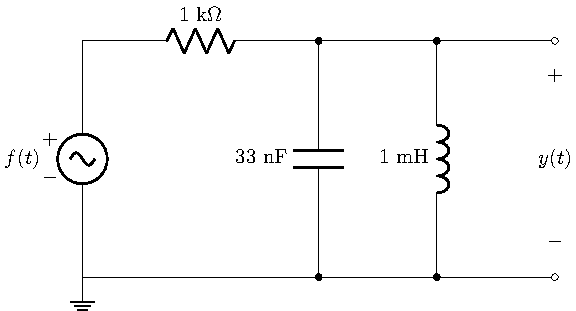
\includegraphics[width=0.7\linewidth]{circuits/circuit_01.pdf}
  \caption{Circuit for analysis in the lab.}
  \label{fig:circuit}
\end{figure}

\begin{figure}[h!]
  \centering
  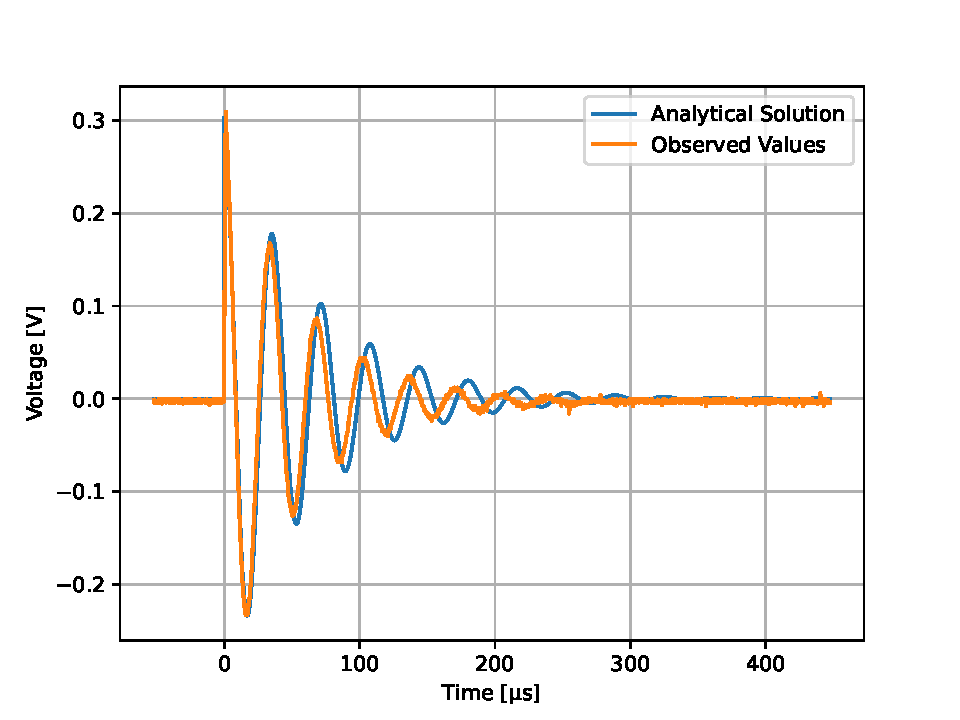
\includegraphics[width=0.7\linewidth]{plots/plot.pdf}
  \caption{Graph of results comparing analytical solution and measured values.}
  \label{fig:plot}
\end{figure}


\end{document}
%%% Local Variables:
%%% mode: latex
%%% TeX-master: t
%%% End:
